\documentclass[12pt]{article}
\usepackage{amsfonts}
\usepackage{amssymb}
\usepackage{homework}

\graphicspath{{../figures/}}

\setlength\fboxsep{0.1em} \setlength\fboxrule{0.5pt}
\sethwtitle{ECE661 Homework6}%
\sethwauthor{Lin Yuan}%
\makehwheader%

\begin{document}
\lstset{language=C++,frame=shadowbox,rulesepcolor=\color{gray},commentstyle=\color{OliveGreen},keywordstyle=\color{blue}\bfseries}
\makehwtitle%

\section{Problem Description}
This homework is about implementing Zhang's algorithm for camera calibration. Besides the techniques from the paper for calculating $K$ and $[R|t]$, we need to use Hough Transform to find lines from the calibration pattern image and then locate the corners, in order to generate the point correspondences automatically.

\section{Solution}
\subsection{Generating Correspondences}
For this homework, we take a camera to shoot multiple pictures of a fixed flat calibration pattern (Fig. \ref{rr}) from multiple positions. Thus the world coordinates of the corners on the calibration pattern is fixed as the same. In order to get the pixel positions of each corner, the following steps are taken:
\begin{itemize}
\item Use Canny edge detector to generate a binary image of the pattern which highlights the edge of the black blocks. (Fig. \ref{rr})
\item Hough Transform is performed on the image first to get the lines. These lines are represented as polar coordinate, and because of noise of image, usually multiple lines can be found, which actually correspond to the same line. (Fig. \ref{rr})
\item These lines are sorted into 2 groups (horizontal and vertical) first depending on their orientations, and then clustered together depending on sampled points' distance on each line (i.e. the parallel gap).
\item After exactly 10 horizontal lines and 8 vertical lines are found, the corners are first located as the crossing of the lines.
\item Then, Harris corner of the image is found and each crossing is relocated to its nearest Harris corner.
\end{itemize}

After these steps, exactly 80 pixel positions will be generated for one image's 80 corner points.

\subsection{Initial estimation of camera parameters}
\subsubsection{Intrinsic Parameters}
The estimation of intrinsic parameters are done in the following steps:
\begin{itemize}
\item For each image, estimate $H$ on the correspondence previously generated using the RANSAC algorithm.
\item Use Zhang's algorithm, section 3.1 to solve for $K$.
\end{itemize}

\subsubsection{Extrinsic Parameters}
After $K$ is estimated, the extrinsic parameters for each $H$, $R$ and $t$ is calculated according to
$H=K[R|t]$. The initial result of $[R | t]$ need to be rescaled according to the norm of $R_1$ and then corrected using the Frobenius method as in Appendic C of Zhang's paper.

\subsubsection{Radial Distortion}
The radial distortion parameters $k1$ and $k2$ are estimated according to Section3.3 of Zhang's paper. We use the estimated intrinsic parameters to generate the equation (13) in Zhang's paper to solve for $k1$ and $k2$.

\subsection{Refining the estimation using LM}
As in last homework, we can refine the parameters $H=K[R_1 R_2 |t]$ using the LM method based on the objective function which is the distance of projected world points with real corner pixel positions. Using the Rodrigues' representation, each rotation matrix $R$ can be represented with only 3 independent parameters. Thus enabling us to use the LM method. So all of parameters for LM are: $u_0,v_0,\alpha,\beta,\gamma,k_1,k_2$ and $6\times n$ extrinsic parameters for $n$ images where in each 6 parameters 3 of them are the Rodrigues representation of $R$, and the other 3 are $t$. The objective function then becomes ${\Vert {\bf x}'- K[R_1 R_2 t]{\bf x}\Vert}^2$ where ${\bf x}'$ is the image corner positions and ${\bf x}$ are the world coordinates of the corners. Sum all the points from all $n$ images, we get $80\times n$ distances added together as the total objective function.

\subsection{Software Structure}
I implemented this homework mostly with C++. For the LM optimization, I did it both in C++ and in MATLAB. The MATLAB code was adapted from last homework, but because it is based on the symbolic toolbox, it is slow and can only perform the optimization for at most 5 images as in the total objective function. For the case that 40 images need to be considered, the levmar package is used in my C++ code. In order to write own LM algorithm in MATLAB that can be applied to 40 images, some tricks like vectorization of the parameters and breaking the calculation of jacobian into parts need to be carried out.

There are several configurations available in my software. All available ways of running the binary hw6 can be found in the file ``test.bash''. All the results (figures) shown below are from the C++ levmar configuration, per the requirement that experiments need to be carried out on at least 20 images. %A package ported with CMake is available at \url{http://web.ics.purdue.edu/~yuanl/download/opencvlevmar.zip} which is good for compiling under Win32+VS, in order that the configuration of levmar package is clear to all of the future references.

\section{Experiences and Discussion}
Through extensive programming work done these days, I'd like to summarize the lessons learned from this experiment.
\begin{itemize}
\item Divide the Hough lines into 2 groups first before merging the lines. Because it is difficult to design a cost function for all orientations of lines. If the lines are initially aligned somehow, the cost function works better. At first I tried to merge the lines first, and then separate them to 2 groups, but the merging didn't work well for all sets of images.
\item When using the Frobenius matrix norm to refine $R$, use only 1 scale factor as $\lambda$, in the last part of Section 3.1 of Zhang's paper. I used $1/\Vert K^{-1}h_1\Vert$ as $\lambda$ and then rescale $t$ also using that $\lambda$. And then $t$ is left there.
\item When using levmar, the distance function provided to levmar must not have memory leak. i.e. All memories allocated inside that function need to be released because that function need to be called many times.
\item When calculating Jacobian in MATLAB using symbols, after calculation, one can store the symbol representation of the Jacobian into a file as a function. So that one do not need to use the $subs$ method which is very slow.
\item According to the last homework, I used my own LM MATLAB code at first. However, it works for at most 5 images. Let alone that I need to generate the MATLAB code of symbols from C++ iteratively, the size of the Jacobian is just intractable, for more than 5 images. So, levmar is suggested for use when you need to optimize on many images, while extra techniques need to be applied to avoid the symbolic toolbox for MATLAB to work for more than 5 images as in the total objective function.
\item My own MATLAB code for this homework is also attached. %, however, because of file size, the generated jacobian is here for download: (for 5 images): \url{http://web.ics.purdue.edu/~yuanl/download/hw6jacobian.zip}
    %Here is the first few lines of a generated jacobian from MATLAB:\\
%\begin{verbatim}returnValue=[[-tx0/tz0,0,-ty0/tz0,-au/tz0,0,0,0,0,-sk/tz0,0,0,0,0,-u0/tz0+(au*tx0+sk*ty0+u0*tz0)/tz0^2,0,0,0,0,-1,0,0,0,0,0,0,0,0,0,0,0,0,0,0,0,0],[0,-ty0/tz0,0,0,0,0,0,0,-av/tz0,0,0,0,0,-v0/tz0+(av*ty0+v0*tz0)/tz0^2,0,0,0,0,0,-1,0,0,0,0,0,0,0,0,0,0,0,0,0,0,0],[-(1+(1-cos((wx0^2+wy0^2+wz0^2)^(1/2)))/(wx0^2+wy0^2+wz0^2)*(-wz0^2-wy0^2)+tx0)/(-sin((wx0^2+wy0^2+wz0^2)^(1/2))/(wx0^2+wy0^2+wz0^2)^(1/2)*wy0+(1-cos((wx0^2+wy0^2+wz0^2)^(1/2)))/(wx0^2+wy0^2+wz0^2)*wz0*wx0+tz0),0,-(sin((wx0^2+wy0^2+wz0^2)^(1/2))/(wx0^2+wy0^2+wz0^2)^(1/2)*wz0+(1-cos((wx0^2+wy0^2+wz0^2)^(1/2)))/(wx0^2+wy0^2+wz0^2)*wy0*wx0+ty0)/(-sin((wx0^2+wy0^2+wz0^2)^(1/2))/(wx0^2+wy0^2+wz0^2)^(1/2)*wy0+(1-cos((wx0^2+wy0^2+wz0^2)^(1/2)))/(wx0^2+wy0^2+wz0^2)*wz0*wx0+tz0),-au/(-sin((wx0^2+wy0^2+wz0^2)^(1/2))/(wx0^2+wy0^2+wz0^2)^(1/2)*wy0+(1-cos((wx0^2+wy0^2+wz0^2)^(1/2)))/(wx0^2+wy0^2+wz0^2)*wz0*wx0+tz0),0,0,0,0,-sk/(-sin((wx0^2+wy0^2+wz0^2)^(1/2))/(wx0^2+wy0^2+wz0^2)^(1/2)*wy0+(1-cos((wx0^2+wy0^2+wz0^2)^(1/2)))/(wx0^2+wy0^2+wz0^2)*wz0*wx0+tz0),0,0,0,0,-u0/(-sin((wx0^2+wy0^2+wz0^2)^(1/2))/(wx0^2+wy0^2+wz0^2)^(1/2)*wy0+(1-cos((wx0^2+wy0^2+wz0^2)^(1/2)))/(wx0^2+wy0^2+wz0^2)*wz0*wx0+tz0)+(au*(1+(1-cos((wx0^2+wy0^2+wz0^2)^(1/2)))/(wx0^2+wy0^2+wz0^2)*(-wz0^2-wy0^2))+sk*(sin((wx0^2+wy0^2+wz0^2)^(1/2))/(wx0^2+wy0^2+wz0^2)^(1/2)*wz0+(1-cos((wx0^2+wy0^2+wz0^2)^(1/2)))/(wx0^2+wy0^2+wz0^2)*wy0*wx0)+u0*(-sin((wx0^2+wy0^2+wz0^2)^(1/2))/(wx0^2+wy0^2+wz0^2)^(1/2)*wy0+(1-cos((wx0^2+wy0^2+wz0^2)^(1/2)))/(wx0^2+wy0^2+wz0^2)*wz0*wx0)+au*tx0+sk*ty0+u0*tz0)/(-sin((wx0^2+wy0^2+wz0^2)^(1/2))/(wx0^2+wy0^2+wz0^2)^(1/2)*wy0+(1-cos((wx0^2+wy0^2+wz0^2)^(1/2)))/(wx0^2+wy0^2+wz0^2)*wz0*wx0+tz0)^2,0,0,0,0,-1,0,-(au*(sin((wx0^2+wy0^2+wz0^2)^(1/2))/(wx0^2+wy0^2+wz0^2)^(3/2)*wx0*(-wz0^2-wy0^2)-2*(1-cos((wx0^2+wy0^2+wz0^2)^(1/2)))/(wx0^2+wy0^2+wz0^2)^2*(-wz0^2-wy0^2)*wx0)+sk*(cos((wx0^2+wy0^2+wz0^2)^(1/2))/(wx0^2+wy0^2+wz0^2)*wx0*wz0-sin((wx0^2+wy0^2+wz0^2)^(1/2))/(wx0^2+wy0^2+wz0^2)^(3/2)*wz0*wx0+sin((wx0^2+wy0^2+wz0^2)^(1/2))/(wx0^2+wy0^2+wz0^2)^(3/2)*wx0^2*wy0-2*(1-cos((wx0^2+wy0^2+wz0^2)^(1/2)))/(wx0^2+wy0^2+wz0^2)^2*wy0*wx0^2+(1-cos((wx0^2+wy0^2+wz0^2)^(1/2)))/(wx0^2+wy0^2+wz0^2)*wy0)+u0*(-cos((wx0^2+wy0^2+wz0^2)^(1/2))/(wx0^2+wy0^2+wz0^2)*wx0*wy0+sin((wx0^2+wy0^2+wz0^2)^(1/2))/(wx0^2+wy0^2+wz0^2)^(3/2)*wy0*wx0+sin((wx0^2+wy0^2+wz0^2)^(1/2))/(wx0^2+wy0^2+wz0^2)^(3/2)*wx0^2*wz0-2*(1-cos((wx0^2+wy0^2+wz0^2)^(1/2)))/(wx0^2+wy0^2+wz0^2)^2*wz0*wx0^2+(1-cos((wx0^2+wy0^2+wz0^2)^(1/2)))/(wx0^2+wy0^2+wz0^2)*wz0))/(-sin((wx0^2+wy0^2+wz0^2)^(1/2))/(wx0^2+wy0^2+wz0^2)^(1/2)*wy0+(1-cos((wx0^2+wy0^2+wz0^2)^(1/2)))/(wx0^2+wy0^2+wz0^2)*wz0*wx0+tz0)+(au*(1+(1-cos((wx0^2+wy0^2+wz0^2)^(1/2)))/(wx0^2+wy0^2+wz0^2)*(-wz0^2-wy0^2))+sk*(sin((wx0^2+wy0^2+wz0^2)^(1/2))/(wx0^2+wy0^2+wz0^2)^(1/2)*wz0+(1-cos((wx0^2+wy0^2+wz0^2)^(1/2)))/(wx0^2+wy0^2+wz0^2)*wy0*wx0)+u0*(-sin((wx0^2+wy0^2+wz0^2)^(1/2))/(wx0^2+wy0^2+wz0^2)^(1/2)*wy0+(1-cos((wx0^2+wy0^2+wz0^2)^(1/2)))/(wx0^2+wy0^2+wz0^2)*wz0*wx0)+au*tx0+sk*ty0+u0*tz0)/(-sin((wx0^2+wy0^2+wz0^2)^(1/2))/(wx0^2+wy0^2+wz0^2)^(1/2)*wy0+(1-cos((wx0^2+wy0^2+wz0^2)^(1/2)))/(wx0^2+wy0^2+wz0^2)*wz0*wx0+tz0)^2*(-cos((wx0^2+wy0^2+wz0^2)^(1/2))/(wx0^2+wy0^2+wz0^2)*wx0*wy0+sin((wx0^2+wy0^2+wz0^2)^(1/2))/(wx0^2+wy0^2+wz0^2)^(3/2)*wy0*wx0+sin((wx0^2+wy0^2+wz0^2)^(1/2))/(wx0^2+wy0^2+wz0^2)^(3/2)*wx0^2*wz0-2*(1-cos((wx0^2+wy0^2+wz0^2)^(1/2)))/(wx0^2+wy0^2+wz0^2)^2*wz0*wx0^2+(1-cos((wx0^2+wy0^2+wz0^2)^(1/2)))/(wx0^2+wy0^2+wz0^2)*wz0),0,0,0,0,-(au*(sin((wx0^2+wy0^2+wz0^2)^(1/2))/(wx0^2+wy0^2+wz0^2)^(3/2)*wy0*(-wz0^2-wy0^2)-2*(1-cos((wx0^2+wy0^2+wz0^2)^(1/2)))/(wx0^2+wy0^2+wz0^2)^2*(-wz0^2-wy0^2)*wy0-2*(1-cos((wx0^2+wy0^2+wz0^2)^(1/2)))/(wx0^2+wy0^2+wz0^2)*wy0)+sk*(cos((wx0^2+wy0^2+wz0^2)^(1/2))/(wx0^2+wy0^2+wz0^2)*wy0*wz0-sin((wx0^2+wy0^2+wz0^2)^(1/2))/(wx0^2+wy0^2+wz0^2)^(3/2)*wz0*wy0+sin((wx0^2+wy0^2+wz0^2)^(1/2))/(wx0^2+wy0^2+wz0^2)^(3/2)*wy0^2*wx0-2*(1-cos((wx0^2+wy0^2+wz0^2)^(1/2)))/(wx0^2+wy0^2+wz0^2)^2*wy0^2*wx0+(1-cos((wx0^2+wy0^2+wz0^2)^(1/2)))/(wx0^2+wy0^2+wz0^2)*wx0)+u0*(-cos((wx0^2+wy0^2+wz0^2)^(1/2))/(wx0^2+wy0^2+wz0^2)*wy0^2+sin((wx0^2+wy0^2+wz0^2)^(1/2))/(wx0^2+wy0^2+wz0^2)^(3/2)*wy0^2-sin((wx0^2+wy0^2+wz0^2)^(1/2))/(wx0^2+wy0^2+wz0^2)^(
%\end{verbatim}
    Some of the corrected images using the my MATLAB LM function is listed on Fig. \ref{mt}
    \begin{figure}[!H]
    \centering
    \subfloat[]{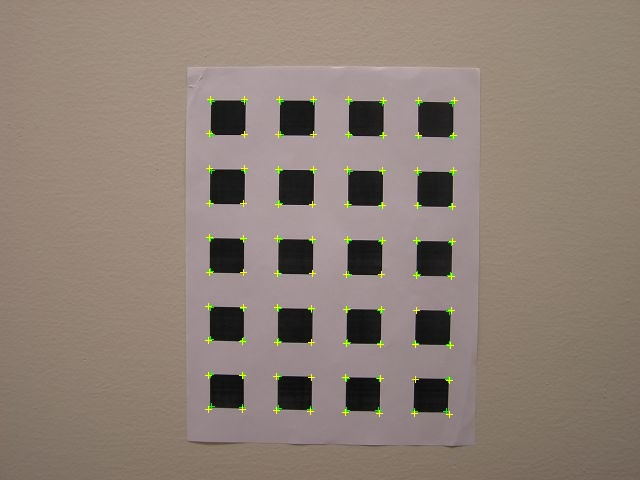
\includegraphics[width=0.4\textwidth]{P1010001s_BP_MATLAB.jpg}}
    \subfloat[]{\includegraphics[width=0.4\textwidth]{P1010001s_BP_BAD_MATLAB.jpg}}
    \caption{MATLAB LM optimization using 5 images only\label{mt}}
    \end{figure}
\end{itemize}

%\section{Code}\footnote{All source/figures available at:
%\url{http://web.ics.purdue.edu/~yuanl/download/EE661}, require your
%Purdue Career Account Login, only the Professor/TA can access it.}
%\label{src} \sffamily\footnotesize%
%test.bash:\\
%\lstinputlisting[breaklines=true]{../../code/src/hw6/test.bash} %
%GENERATEJac.m
%\lstinputlisting[language=MATLAB,breaklines=true]{../../code/src/hw6/GENERATEJac.m} %
%GENERATEallH.m
%\lstinputlisting[language=MATLAB,breaklines=true]{../../code/src/hw6/GENERATEallH.m} %
%NONLINEAROPTby.m
%\lstinputlisting[language=MATLAB,breaklines=true]{../../code/src/hw6/NONLINEAROPTby.m} %
%hw6.cpp:\\
%\lstinputlisting[language=C++,breaklines=true]{../../code/src/hw6/hw6.cpp} %
%checkerby.h:\\
%\lstinputlisting[language=C++,breaklines=true]{../../code/src/hw6/checkerby.h} %
%checkerby.cpp:\\
%\lstinputlisting[language=C++,breaklines=true]{../../code/src/hw6/checkerby.cpp} %
%zhengyouby.h:\\
%\lstinputlisting[language=C++,breaklines=true]{../../code/src/hw6/zhengyouby.h} %
%zhengyouby.cpp:\\
%\lstinputlisting[language=C++,breaklines=true]{../../code/src/hw6/zhengyouby.cpp} %
%levmarby.h:\\
%\lstinputlisting[language=C++,breaklines=true]{../../code/src/hw6/levmarby.h} %
%levmarby.cpp:\\
%\lstinputlisting[language=C++,breaklines=true]{../../code/src/hw6/levmarby.cpp} %
%CMakeLists.txt:\\
%\lstinputlisting[breaklines=true]{../../code/CMakeLists.txt} %
%\rmfamily\normalsize

\section{Results}
\tiny
\begin{table}[!h]
\centering
\begin{tabular}{|c|c|c|}
\hline
 & Initial & Refined \\
\hline
$K$ & $
\left( {\begin{array}{*{20}c}
   {717.359251} & {1.582683} & {324.590701}  \\
   {0} & {718.503845} & {237.299279}  \\
   {0} & {0} & {1}  \\
\end{array}} \right)
$
& $
\left( {\begin{array}{*{20}c}
   {731.435860} & {2.014288} & {320.486042}  \\
   {0} & {733.096893} & {240.158381}  \\
   {0} & {0} & {1}  \\
\end{array}} \right)
$\\
\hline
$R_1$ & $
\left( {\begin{array}{*{20}c}
   {0.999410} & {-0.012255} & {0.032091}  \\
   {0.013624} & {0.998991} & {-0.042801}  \\
   {-0.031534} & {0.043213} & {0.998568}  \\
\end{array}} \right)
$ & $
\left( {\begin{array}{*{20}c}
   {0.999159} & {-0.012466} & {0.039061}  \\
   {0.013768} & {0.999353} & {-0.033221}  \\
   {-0.038621} & {0.033730} & {0.998684}  \\
\end{array}} \right)
$\\
\hline
$t_1$ & $
\left( {\begin{array}{*{20}c}
   {-3.299247}  \\
   {-3.979002}  \\
   {20.786686}  \\
\end{array}} \right)
$
& $
\left( {\begin{array}{*{20}c}
   {-3.177474}  \\
   {-4.066574}  \\
   {21.101353 }  \\
\end{array}} \right)
$
\\
\hline
D & (0.098037,-1.639184) &(-0.201687 0.039493) \\
\hline
F & 7429.61 & 3771.05 \\
\hline
\end{tabular}
\caption{Parameters For Image Set 1, R,t for image P1010001s.jpg}
\end{table}
\begin{table}[!h]
\centering
\begin{tabular}{|c|c|c|}
\hline
 & Initial & Refined \\
\hline
$K$ & $
\left( {\begin{array}{*{20}c}
   {644.667493} & {-3.084936} & {324.993269}  \\
   {0} & {646.253247} & {245.778708}  \\
   {0} & {0} & {1}  \\
\end{array}} \right)
$
& $
\left( {\begin{array}{*{20}c}
   {638.467493} & {-3.956473} & {323.982361}  \\
   {0} & {639.516005} & {250.617438}  \\
   {0} & {0} & {1}  \\
\end{array}} \right)
$\\
\hline
$R_1$ & $
\left( {\begin{array}{*{20}c}
   {0.996199} & {0.011029} & {-0.086402}  \\
   {-0.015785} & {0.998386} & {-0.054560}  \\
   {0.085661} & {0.055716} & {0.994765}  \\
\end{array}} \right)
$ & $
\left( {\begin{array}{*{20}c}
   {0.996304} & {0.011689} & {-0.085095}  \\
   {-0.016630} & {0.998202} & {-0.057588}  \\
   {0.084269} & {0.058790} & {0.994707}  \\
\end{array}} \right)
$\\
\hline
$t_1$ & $
\left( {\begin{array}{*{20}c}
   {-4.320643}  \\
   {-4.884312}  \\
   {18.535515}  \\
\end{array}} \right)
$
& $
\left( {\begin{array}{*{20}c}
   {-4.304821}  \\
   {-5.046637}  \\
   {18.430106}  \\
\end{array}} \right)
$
\\
\hline
D & (0.033083,-0.394379) & (0.112342,-0.941011) \\
\hline
F & 3264.81 & 2634.34 \\
\hline
\end{tabular}
\caption{Parameters For Image Set 2, R,t for image IMG-20101111-00032.jpg}
\end{table}
\normalsize
\begin{figure}[!h]
\centering
\subfloat[Canny Image]{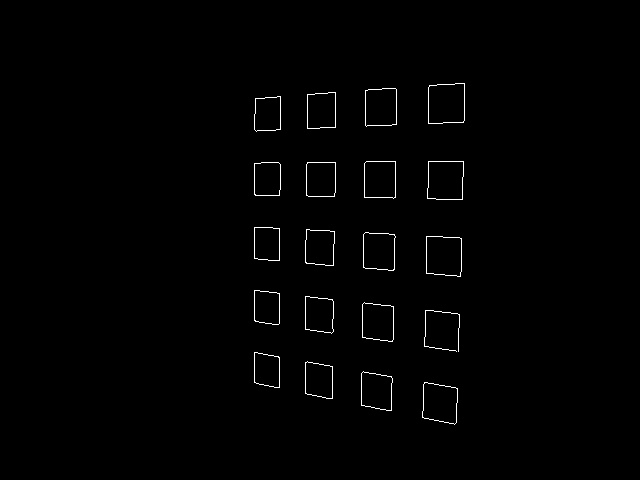
\includegraphics[height=0.22\textheight]{canny}}%
\subfloat[Hough Lines]{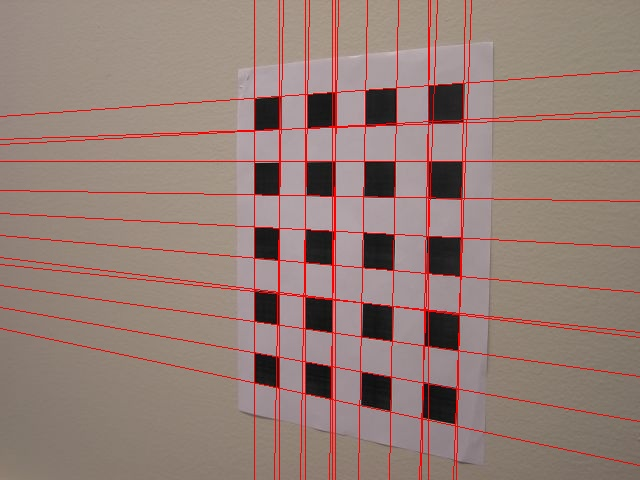
\includegraphics[height=0.22\textheight]{imageBad}}\\%
\subfloat[Merged Horizontal Lines]{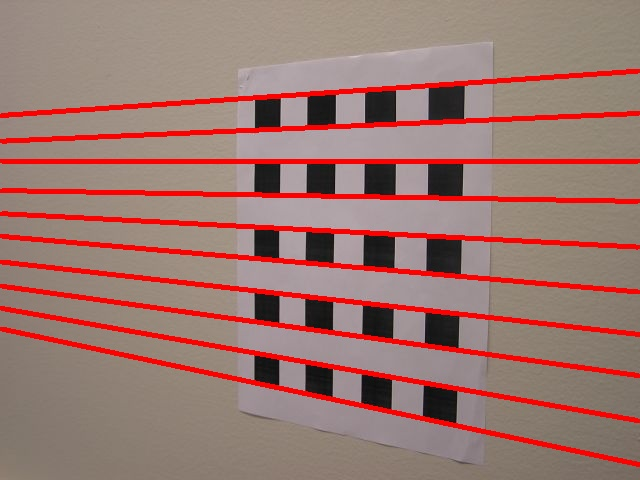
\includegraphics[height=0.22\textheight]{imageHor}}
\subfloat[Merged Vertical Lines]{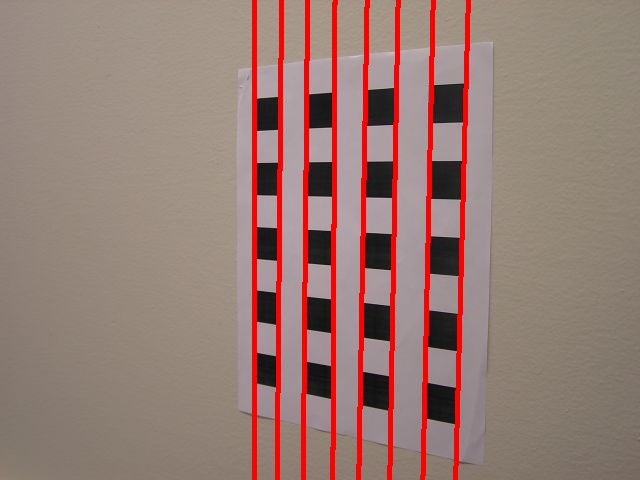
\includegraphics[height=0.22\textheight]{imageVer}}\\
\subfloat[Final Line Set]{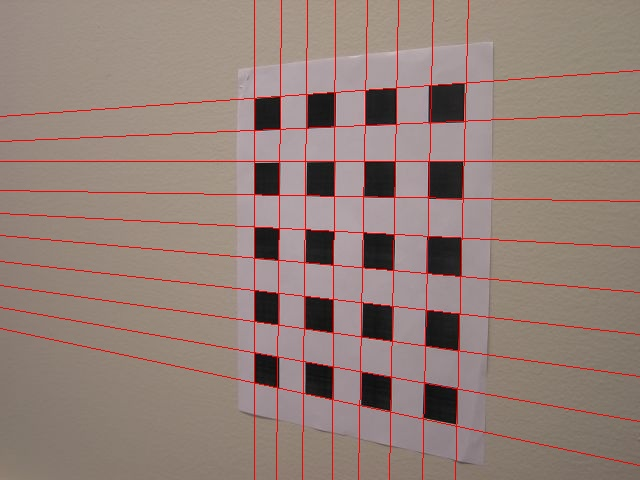
\includegraphics[height=0.22\textheight]{imageH}}
\subfloat[Labeled Corners]{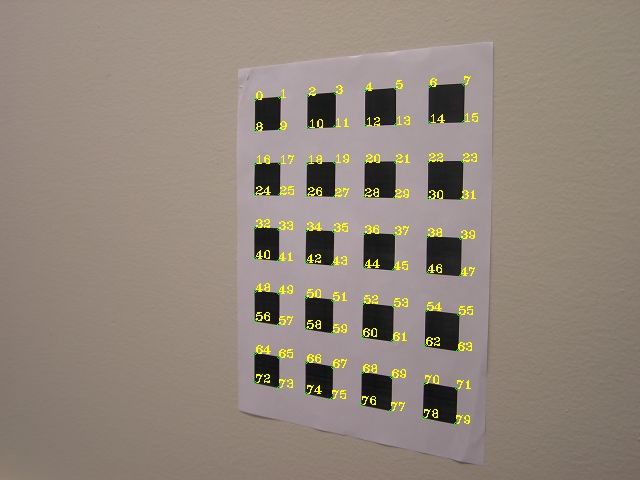
\includegraphics[height=0.22\textheight]{imageCorner}}\\
\caption{Intermediate results\label{rr}}
\end{figure}
\begin{figure}[!h]
\centering
\subfloat[Initial Parameters Reprojected]{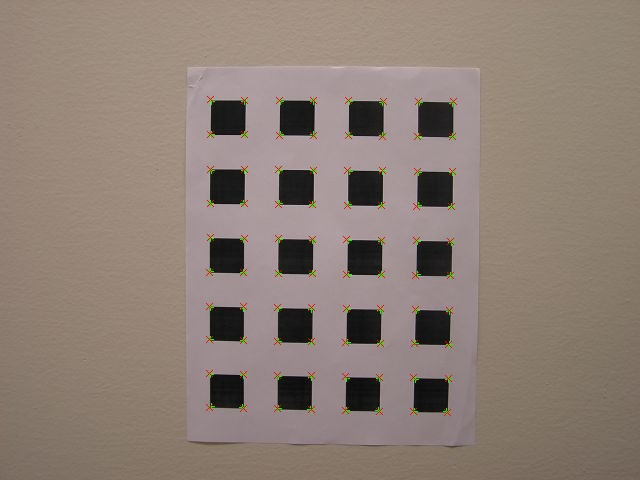
\includegraphics[height=0.4\textheight]{P1010001s_BP_Bad.jpg}}\\
\subfloat[Refined Parameters Reprojected]{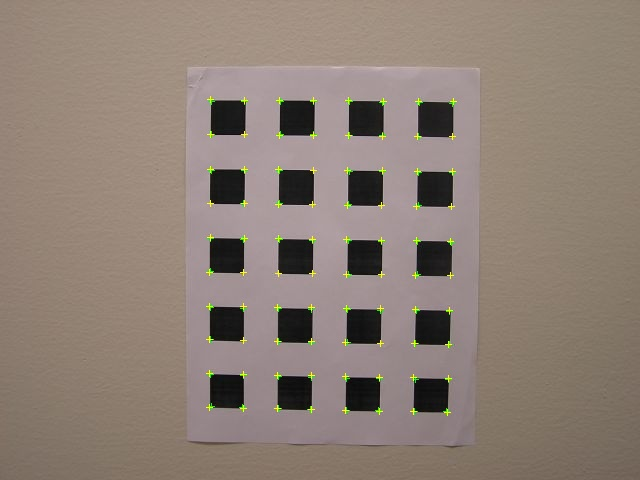
\includegraphics[height=0.4\textheight]{P1010001s_BP.jpg}}\\
\caption{Image Set 1}
\end{figure}
\begin{figure}[!h]
\centering
\subfloat[Initial Parameters Reprojected]{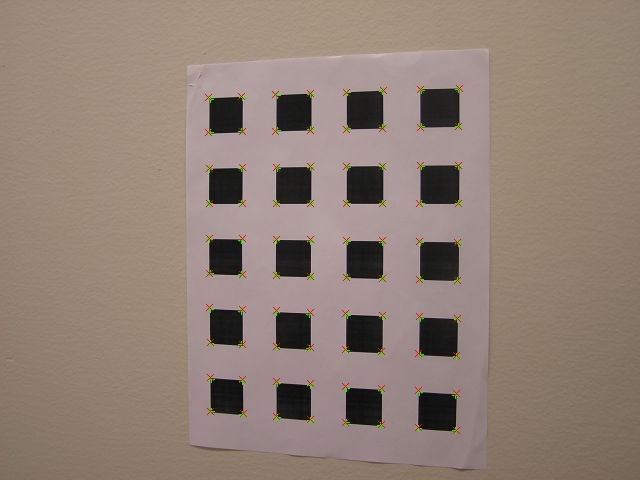
\includegraphics[height=0.4\textheight]{P1010002s_BP_Bad.jpg}}\\
\subfloat[Refined Parameters Reprojected]{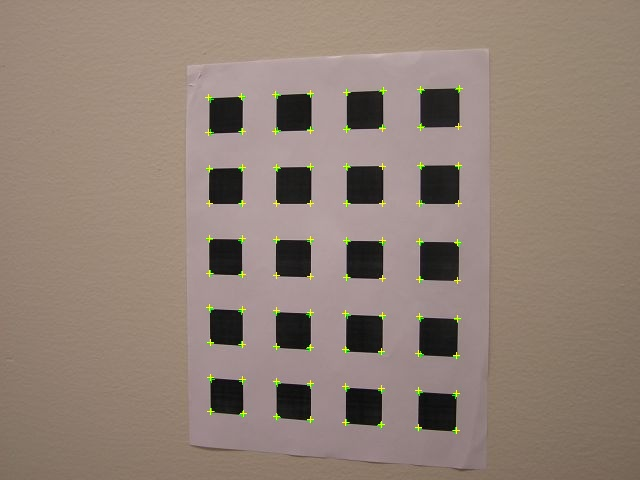
\includegraphics[height=0.4\textheight]{P1010002s_BP.jpg}}\\
\caption{Image Set 1}
\end{figure}
\begin{figure}[!h]
\centering
\subfloat[Initial Parameters Reprojected]{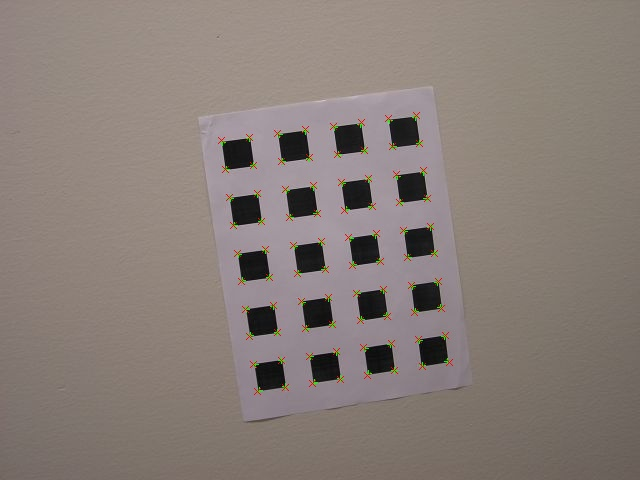
\includegraphics[height=0.4\textheight]{P1010015s_BP_Bad.jpg}}\\
\subfloat[Refined Parameters Reprojected]{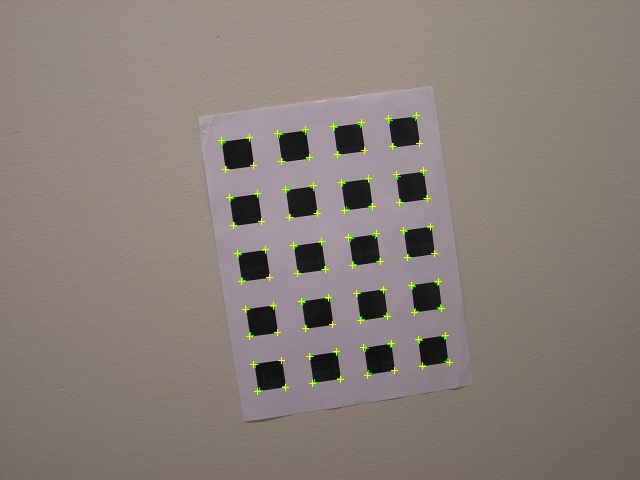
\includegraphics[height=0.4\textheight]{P1010015s_BP.jpg}}\\
\caption{Image Set 1}
\end{figure}

\begin{figure}[!h]
\centering
\subfloat[Initial Parameters Reprojected]{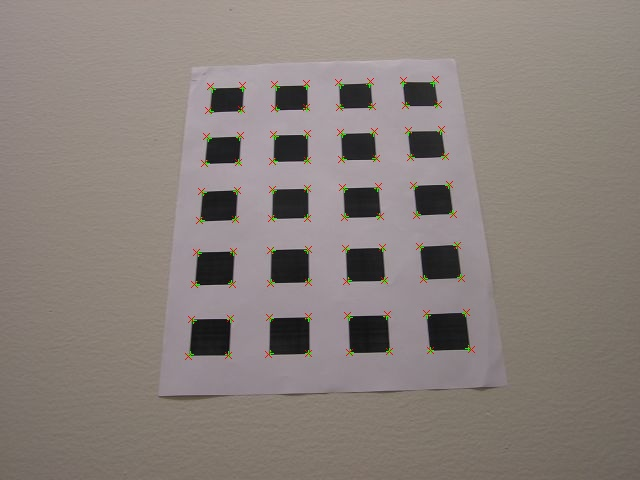
\includegraphics[height=0.4\textheight]{P1010016s_BP_Bad.jpg}}\\
\subfloat[Refined Parameters Reprojected]{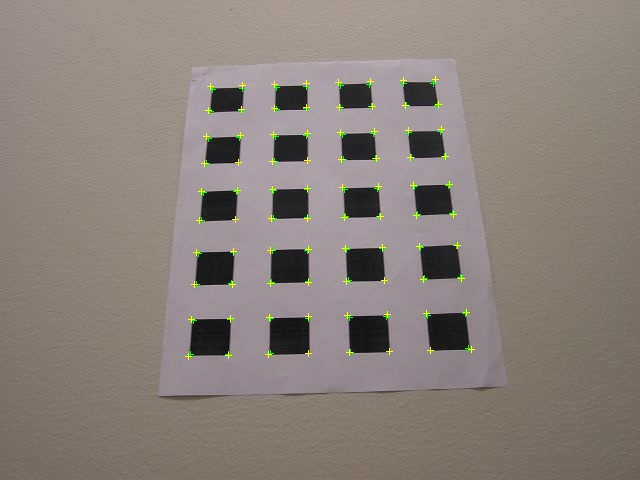
\includegraphics[height=0.4\textheight]{P1010016s_BP.jpg}}\\
\caption{Image Set 1}
\end{figure}
\begin{figure}[!h]
\centering
\subfloat[Initial Parameters Reprojected]{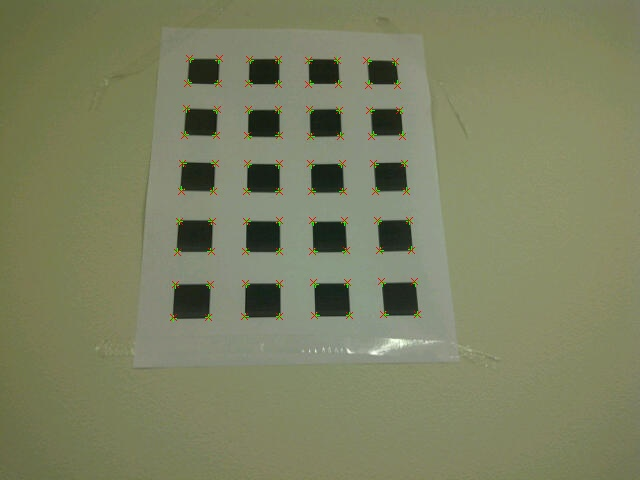
\includegraphics[height=0.4\textheight]{IMG-20101111-00034_BP_Bad.jpg}}\\
\subfloat[Refined Parameters Reprojected]{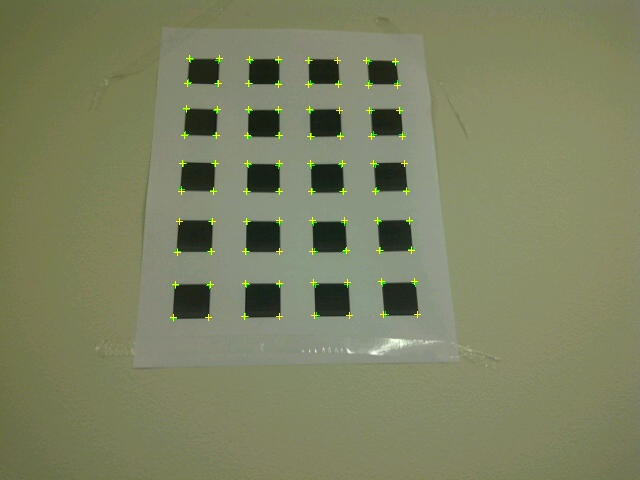
\includegraphics[height=0.4\textheight]{IMG-20101111-00034_BP.jpg}}\\
\caption{Image Set 2}
\end{figure}
\begin{figure}[!h]
\centering
\subfloat[Initial Parameters Reprojected]{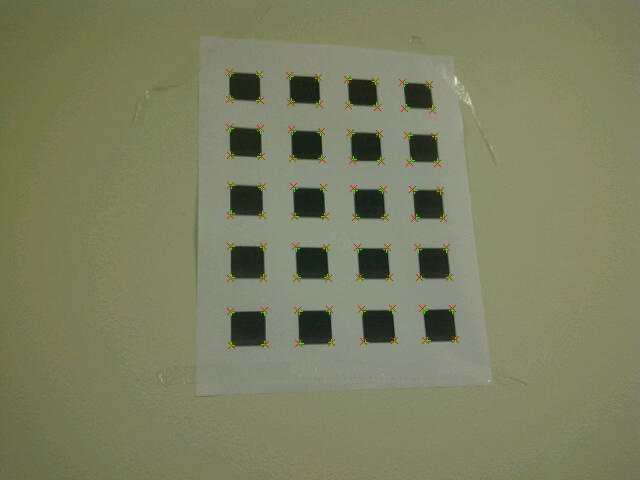
\includegraphics[height=0.4\textheight]{IMG-20101111-00036_BP_Bad.jpg}}\\
\subfloat[Refined Parameters Reprojected]{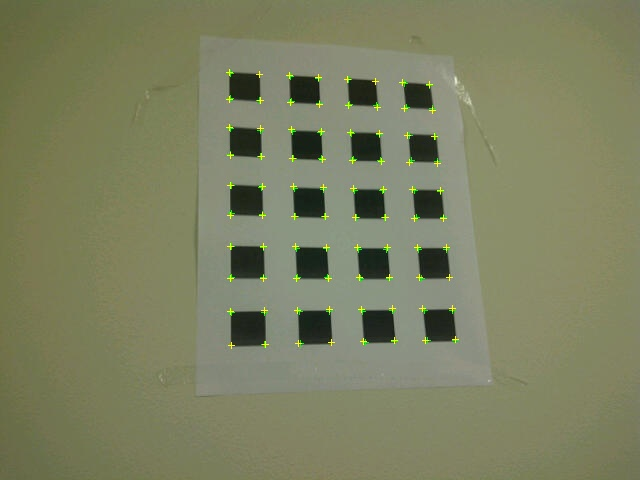
\includegraphics[height=0.4\textheight]{IMG-20101111-00036_BP.jpg}}\\
\caption{Image Set 2}
\end{figure}
\begin{figure}[!h]
\centering
\subfloat[Initial Parameters Reprojected]{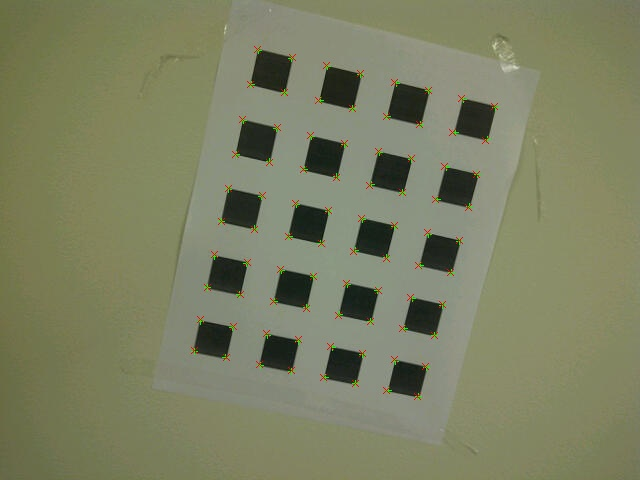
\includegraphics[height=0.4\textheight]{IMG-20101111-00053_BP_Bad.jpg}}\\
\subfloat[Refined Parameters Reprojected]{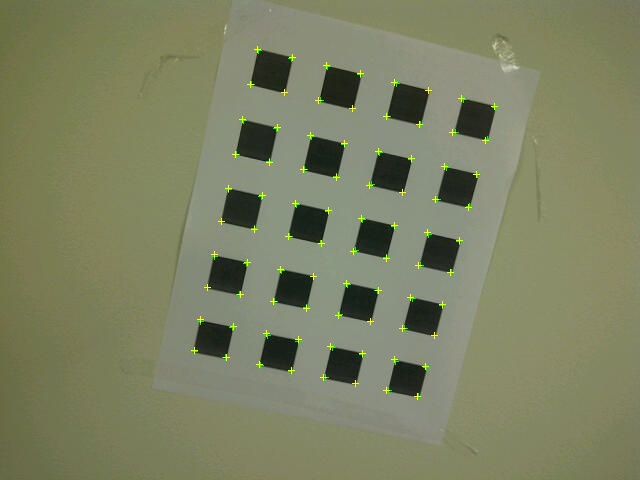
\includegraphics[height=0.4\textheight]{IMG-20101111-00053_BP.jpg}}\\
\caption{Image Set 2}
\end{figure}
\begin{figure}[!h]
\centering
\subfloat[Initial Parameters Reprojected]{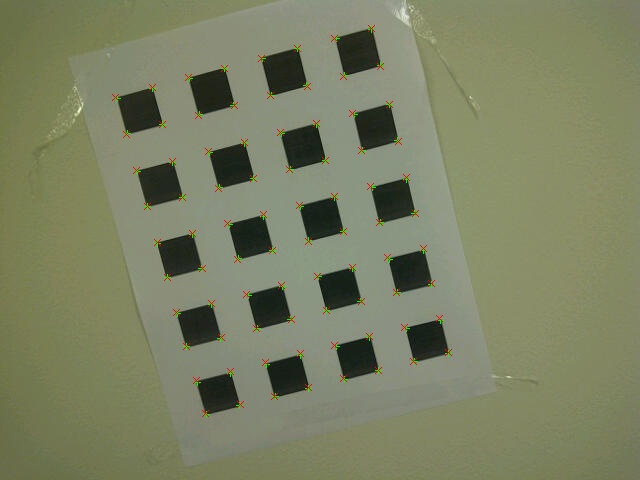
\includegraphics[height=0.4\textheight]{IMG-20101111-00055_BP_Bad.jpg}}\\
\subfloat[Refined Parameters Reprojected]{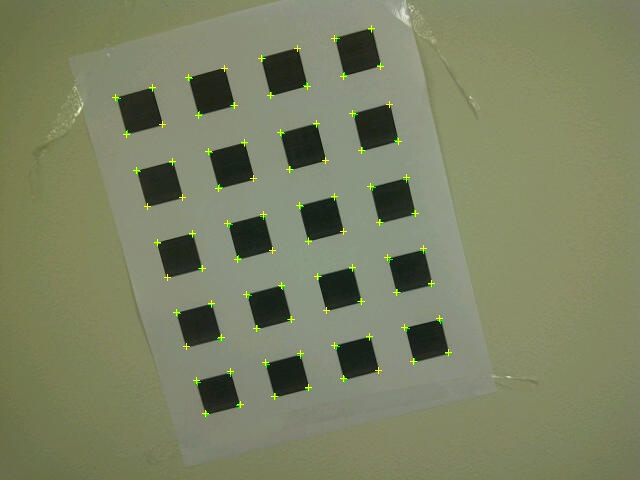
\includegraphics[height=0.4\textheight]{IMG-20101111-00055_BP.jpg}}\\
\caption{Image Set 2}
\end{figure}


\end{document}
